\documentclass[Lecture.tex]{subfiles}
\begin{document}
\section{5.2: The Definite Integral}
\begin{frame}{The Definite Integral}
  \begin{itemize}
  \item<1->
    In the last section, we saw that for a continuous function $f$ on an interval $[a,b]$, the error for Left-Hand Sums and Right-Hand Sums goes to zero as the number of points in the partition becomes large.
  \item<2->
    As the error term goes to zero, the Left-Hand Sum increases towards a fixed value and the Right-Hand Sum decreases towards that same value.
  \item<3->
    The common value that these sums approach is called a {\it limit}, and we call this particular limit the Definite Integral.
  \end{itemize}
\end{frame}

\begin{frame}{Formal Definition of the Definite Integral}
  \begin{defn}
    Assume that $f$ is continuous on the interval $[a,b]$.
    The {\it definite integral of $f$ from $a$ to $b$} is
    $$\int_a^b f(t)\operatorname{d}t = \lim_{n \rightarrow \infty} \sum_{i = 0}^n f(t_i)\Delta t = \lim_{n \rightarrow \infty} \sum_{i = 1}^n f(t_i)\Delta t,$$
    where the set of $t$-values 
    $$a = t_0 < t_1 < \cdots < t_{n-1} < t_n = b$$
    is a partition of $[a,b]$ into $n$ intervals of length
    $$\Delta t = \frac{b - a}{n}.$$
  \end{defn}
\end{frame}

\begin{frame}{Geometric Examples}
  Compute $\int_{x_0}^{x_1}b \operatorname{d}x$ for $0 < b$.\\
  \vfill
  \begin{minipage}[t]{\linewidth}
    \onslide<2->{
      The integral is just the area of the shaded region below:
    }
    \onslide<3->{
      \begin{center}
        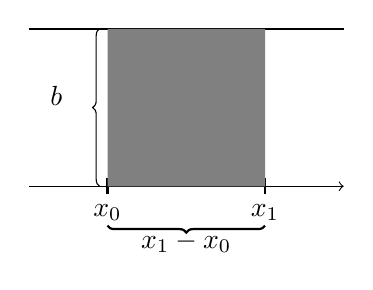
\begin{tikzpicture}
          \draw[-](0,0) -- (1,0);
          \draw[-](1,0) -- (2,0);
          \draw[-](2,0) -- (3,0);
          \draw[->](3,0) -- (4,0);
          \draw[-][thick](0,2) -- (4,2);
          \draw [thick] (1,-.1) node[below]{$x_0$} -- (1,.1);
          \draw [thick] (3,-.1) node[below]{$x_1$} -- (3,.1);
          \path [fill=gray] (1,0) -- (1,2) -- (3,2) -- (3,0) -- (1,0);
          \draw [
            decoration={
              brace,
              raise=0.1cm
            },
            decorate
          ]
          (1,0) -- (1,2) node[pos=.7,anchor=north,xshift=-.65cm]{$b$};
          \draw [
            thick,
            decoration={
              brace,
              mirror,
              raise=0.5cm
            },
            decorate
          ]
          (1,0) -- (3,0) node[pos=0.5,anchor=north,yshift=-.45cm]{$x_1 - x_0$};
        \end{tikzpicture}
      \end{center}
    }
    \onslide<4->{
      $$\int_{x_0}^{x_1} b \operatorname{d}x = b(x_1 - x_0).$$
    }
  \end{minipage}
\end{frame}

\begin{frame}{Geometric Examples}
  Let $f(x) = mx + b$ for $0 < b$, $0 < m$.
  Compute $\int_{x_0}^{x_1}f(x) \operatorname{d}x$ for $\frac{-b}{m} < x_0$.\\
  \vfill
  \begin{minipage}[t]{\linewidth}
    \onslide<2->{
      The integral is just the area of the shaded region below:
    }
    \onslide<3->{
      \begin{center}
        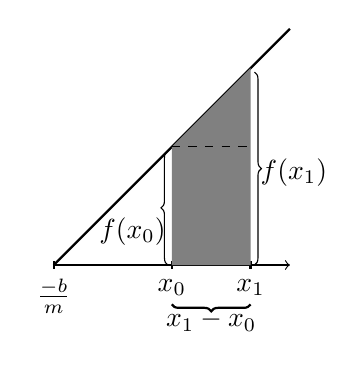
\begin{tikzpicture}[scale=0.5]
          \draw[-](0,0) -- (1,0);
          \draw[-](1,0) -- (2,0);
          \draw[-](2,0) -- (3,0);
          \draw[->](-2,0) -- (4,0);
          \draw[-][thick](-2,0) -- (4,6);
          \draw [thick] (1,-.1) node[below]{$x_0$} -- (1,.1);
          \draw [thick] (-2,-.1) node[below]{$\frac{-b}{m}$} -- (-2,.1);
          \draw [thick] (3,-.1) node[below]{$x_1$} -- (3,.1);
          \path [fill=gray] (1,0) -- (1,3) -- (3,5) -- (3,0) -- (1,0);
          \draw[-][dashed](1,3) -- (3,3);
          \draw [
            decoration={
              brace,
              raise=0.05cm
            },
            decorate
          ]
          (1,0) -- (1,2.9) node[pos=.5,anchor=north,xshift=-.5cm]{$f(x_0)$};
          \draw [
            decoration={
              brace,
              mirror,
              raise=0.05cm
            },
            decorate
          ]
          (3,0) -- (3,4.9) node[pos=.6,anchor=north,xshift=.55cm]{$f(x_1)$};
          \draw [
            thick,
            decoration={
              brace,
              mirror,
              raise=0.5cm
            },
            decorate
          ]
          (1,0) -- (3,0) node[pos=0.5,anchor=north,yshift=-.45cm]{$x_1 - x_0$};
        \end{tikzpicture}
      \end{center}
    }
    \onslide<4->{
      $$\int_{x_0}^{x_1}f(x) \operatorname{d}x = \onslide<5->{f(x_0)(x_1 - x_0) +} \onslide<6->{\frac{1}{2}\left[f(x_1) - f(x_0)\right](x_1 - x_0).}$$
    }
  \end{minipage}
\end{frame}

\begin{frame}{Geometric Examples}
  Compute $\int_{-1}^1 \sqrt{1 - x^2}\operatorname{d}x.$
  \begin{minipage}[t]{\linewidth}
    \begin{itemize}
    \item<2->
      Observe
      $x^2 + y^2 = 1$
      is a circle of radius 1 centered at $(0,0)$ and the area of a cirlce of radius $r$ is
      $\pi \cdot r^2$.
    \item<3->
      The curve $y = \sqrt{1 - x^2}$ is the top half of this circle, and the integral is the area bounded by this semicircle:
      \onslide<4->{
        \begin{center}
          \begin{tikzpicture}[scale=0.5]
            \begin{scope}
              \clip (-1,0) rectangle (1,1);
              \draw [fill = gray] (0,0) circle (1);
            \end{scope}
            \draw [dashed] (0,0) circle (1);
            \draw [->] (-2,0) -- (2,0);
            \draw [->] (0,-2) -- (0,2);
            \node[above right=1mm of {(.707,.707)}] {$y = \sqrt{1 - x^2}$};
          \end{tikzpicture}
        \end{center}
      }
    \item<5->
      Therefore 
      $$\int_{-1}^1 \sqrt{1 - x^2}\operatorname{d}x = \frac{1}{2}\pi(1)^2 = \frac{\pi}{2}.$$
    \end{itemize}
  \end{minipage}
\end{frame}

\begin{frame}{Geometric Examples}
  The area under the parabola
  \begin{center}
    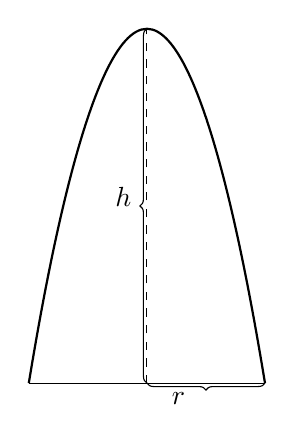
\begin{tikzpicture}[scale=0.5]
      \draw [thick] (-3,0) parabola bend (0,9) (3,0);
      \draw [dashed] (0,0) -- (0,9);
      \draw [-] (-3,0) -- (3,0);
      \draw [
        decoration={
          brace%,
          %raise=0.1cm
        },
        decorate
      ]
      (0,0) -- (0,9) node[pos=.58,anchor=north,xshift=-.3cm]{$h$};
      \draw [
        decoration={
          brace,
          %raise=0.1cm
          mirror
        },
        decorate
      ]
      (0,0) -- (3,0) node[pos=.7,anchor=north,xshift=-.65cm]{$r$};
    \end{tikzpicture}
  \end{center}
  is $\frac{4}{3}rh$.
  Use this to compute $\int_0^3 x^2\operatorname{d}x$.
\end{frame}

\begin{frame}{Geometric Examples}
  The integral is just the area under the parabola:
  \begin{center}
    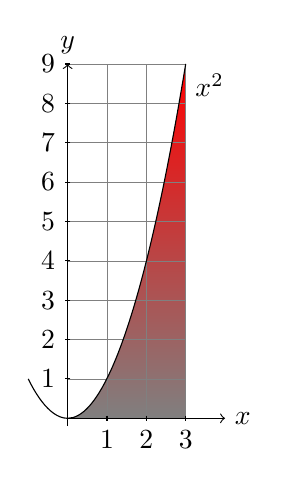
\begin{tikzpicture}[scale = 0.5]
      \shade[top color=red,bottom color = black!50] (0,0) parabola (3,9) |- (0,0);
      %\shade[top color=black,bottom color = red!50] (0,0) parabola (-3,9) |- (0,0);
      \draw[style=help lines] (0,0) grid (3,9) [step = 0.25cm];

      %\draw[->](-3,0) -- (4,0) node[right] {$x$};
      \draw[->](0,0) -- (4,0) node[right] {$x$};
      \draw[->](0,-.2) -- (0,9) node[above] {$y$};
      
      \foreach \x/\xtext in {1/1, 2/2, 3/3}
      \draw[shift={(\x,0)}] (0pt,2pt) -- (0pt,-2pt) node[below] {$\xtext$};
      
      \foreach \y/\ytext in {1/1,2/2,3/3,4/4,5/5,6/6,7/7,8/8,9/9}
      \draw[shift={(0,\y)}] (2pt,0pt) -- (-2pt,0pt) node[left] {$\ytext$};

      %\draw (-3,9) parabola bend (0,0) (3,9) node[below right] {$x^2$};
      \draw (-1,1) parabola bend (0,0) (3,9) node[below right] {$x^2$};
    \end{tikzpicture}
  \end{center}
\end{frame}

\begin{frame}{Geometric Examples}
  If we flip the picture upside down, we have the picture
  \begin{center}
    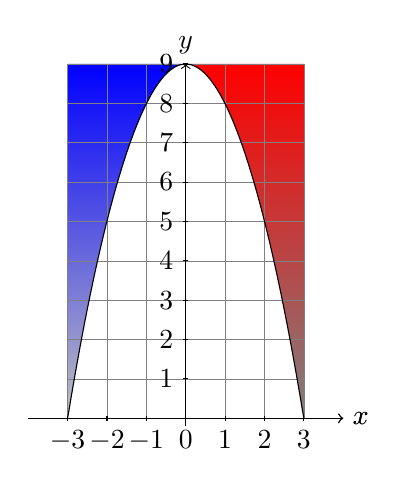
\begin{tikzpicture}[scale = 0.5]
      \path [shade, top color = red, bottom color = black!50] (3,0) -- (3,9) -- (0,9) parabola (3,0);
      \path [shade, top color = blue, bottom color = gray!50] (-3,0) -- (-3,9) -- (0,9) parabola (-3,0);
      \draw[style=help lines] (-3,0) grid (3,9) [step = 0.25cm];

      \draw[->](-4,0) -- (4,0) node[right] {$x$};
      \draw[->](0,0) -- (4,0) node[right] {$x$};
      \draw[->](0,-.2) -- (0,9) node[above] {$y$};
      
      \foreach \x/\xtext in {-3/-3, -2/-2, -1/-1,0/0,1/1,2/2,3/3}
      \draw[shift={(\x,0)}] (0pt,2pt) -- (0pt,-2pt) node[below] {$\xtext$};
      
      \foreach \y/\ytext in {1/1,2/2,3/3,4/4,5/5,6/6,7/7,8/8,9/9}
      \draw[shift={(0,\y)}] (2pt,0pt) -- (-2pt,0pt) node[left] {$\ytext$};

      \draw (-3,0) parabola bend (0,9) (3,0);
    \end{tikzpicture}
  \end{center}
  And we note that the red and blue areas are, by symmetry, the same. 
\end{frame}

\begin{frame}{Geometric Examples}
  Hence we can compute the area using
  \scalebox{0.8}{\parbox{\linewidth}{
  \begin{eqnarray*}
    \onslide<2->{\operatorname{area}\left(
  
\begin{tikzpicture}[scale=0.5]
    \path [shade, top color = red, bottom color = black!50] (1,0) -- (1,1) -- (0,1) parabola (1,0);
  \end{tikzpicture}\right)
  &=&} \onslide<3->{\operatorname{area}\left(
  \begin{tikzpicture}[scale = 0.5]
    \draw (0,0) -- (0,1) -- (1,1) -- (1,0) -- (0,0);
  \end{tikzpicture}\right)
  - \operatorname{area}
  \left(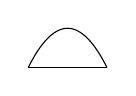
\begin{tikzpicture}[scale = 0.5]
    \draw (-1,0) parabola bend (0,1) (1,0);
    \draw (-1,0) -- (1,0);
  \end{tikzpicture}\right)
  - \operatorname{area}
  \left(
\begin{tikzpicture}[scale = 0.5]
    \path [shade, top color = blue, bottom color = gray!50] (-1,0) -- (-1,1) -- (0,1) parabola (-1,0);
  \end{tikzpicture}\right)\\}
    \onslide<4->{&=& \operatorname{area}\left(
  \begin{tikzpicture}[scale = 0.5]
    \draw (0,0) -- (0,1) -- (1,1) -- (1,0) -- (0,0);
  \end{tikzpicture}\right)
  - \operatorname{area}
  \left(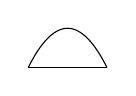
\begin{tikzpicture}[scale = 0.5]
    \draw (-1,0) parabola bend (0,1) (1,0);
    \draw (-1,0) -- (1,0);
  \end{tikzpicture}\right)
  - \operatorname{area}
  \left(
  
\begin{tikzpicture}[scale=0.5]
    \path [shade, top color = red, bottom color = black!50] (1,0) -- (1,1) -- (0,1) parabola (1,0);
  \end{tikzpicture}\right)\\}
    \onslide<5->{\Rightarrow 2 \cdot \operatorname{area}
  \left(
\begin{tikzpicture}[scale=0.5]
    \path [shade, top color = red, bottom color = black!50] (1,0) -- (1,1) -- (0,1) parabola (1,0);
  \end{tikzpicture}\right)
  &=& \operatorname{area}
  \left(\begin{tikzpicture}[scale = 0.5]
    \draw (0,0) -- (0,1) -- (1,1) -- (1,0) -- (0,0);
  \end{tikzpicture}\right)
  - \operatorname{area}
  \left(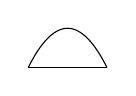
\begin{tikzpicture}[scale = 0.5]
    \draw (-1,0) parabola bend (0,1) (1,0);
    \draw (-1,0) -- (1,0);
  \end{tikzpicture}\right).}
  \end{eqnarray*}
  }}

  \onslide<6->{Therefore}
  \begin{eqnarray*}
    \onslide<7->{\int_0^3 x^2\operatorname{d}x &=&}\onslide<8->{\frac{1}{2}\left[ 6\cdot 9 - \frac{4}{3}\cdot 9 \cdot 3\right]\\}
    \onslide<9->{&=& \frac{1}{2}\left[6\cdot 9\left(1 - \frac{2}{3}\right)\right]\\}
    \onslide<10->{&=& 9.}
    %&=& 3 \cdot 9 \cdot \frac{1}{3}\\
    %&=& 9.
  \end{eqnarray*}
\end{frame}

\end{document}
